\chapter{Study of the Wobbling Motion via a Boson Description}
\label{extra-chapter-new-boson}

The last part will be focused on the same wobbling phenomenon but with a different approach than the ones employed in Chapters \ref{chapter-4-aw1-formalism} and \ref{chapter-5-novel}, as this method does not share the same foundational concepts as the $\mathbf{W_1}$ and $\mathbf{W_2}$ techniques. The results shown here correspond to a recent publication made by the team in Ref. \cite{raduta2020new}. The structure of the chapter is organized as follows: in the first section a set of results achieved by the $\mathbf{W_0}$ formalism are briefly recalled, as some key features from that work will be used throughout this chapter. 
%TO-DO: finish summary of chapter 6.

\section{Angular Momentum - Boson Representation}
\label{section-intro-boson-representation}

Besides the odd-mass case-study performed by the team in Ref. \cite{raduta2017semiclassical}, the first part consisted in describing wobbling motion for even-even nuclei using a \emph{boson expansion} of the angular momentum components. The problem considered a triaxial rigid rotor with moments of inertia $\mathcal{I}_k$, which described by the known rotor Hamiltonian (recall Section \ref{trm-model} and Eq. \ref{general-rotor-hamiltonian}):
\begin{align}
    \hat{H}_R=\frac{\hat{R}_1}{2\mathcal{I}_1}+\frac{\hat{R}_2}{2\mathcal{I}_2}+\frac{\hat{R}_3}{2\mathcal{I}_3}\ ,
\end{align}
and angular momentum components $\hat{R}_k$. From this initial quantal problem, a variational principle (similar recipe as the one described in Section \ref{variational-principle-section}, but only for one set of coordinates) brings the system into a classical view, where the eigenvalue problem becomes a system of classical equations in a phase space (see Section II.A and II.B from Ref. \cite{raduta2017semiclassical}). Summarizing the calculations, one obtained $i)$ a pair of conjugate variables (i.e., $r$ and $\varphi$) and $ii)$ two equations of motion (recall discussion from Section \ref{equations-of-motion-section} and Eq. \ref{eq-of-motion-approach-w1}) as:
\begin{align}
    \frac{\partial\mathcal{H}}{\partial r}=\dot{\varphi}\ ,\ \frac{\partial\mathcal{H}}{\partial\varphi}=-\dot{r}\ ,
\end{align}
with $\mathcal{H}$ as the average of $\hat{H}_R$ with the trial function. If the average values of the angular momentum components are expressed in terms of the phase space coordinates $(r,\varphi)$, then the following equations emerge:
\begin{align}
    J_+^\text{cls}&\equiv\langle\hat{R}_+\rangle=\sqrt{r(2I-r)}e^{\iu\varphi}\ ,\nonumber \\
    J_-^\text{cls}&\equiv\langle\hat{R}_-\rangle=\sqrt{r(2I-r)}e^{-\iu\varphi}\ ,\nonumber \\
    J_3^\text{cls}&\equiv\langle\hat{R}_3\rangle=r-I\ .
    \label{classical-am-components-boson}
\end{align} 

Their algebra being governed by the Poisson brackets, which defines their inner product:
\begin{align}
    \left\{J_+^\text{cls},J_-^\text{cls}\right\}=-2\iu J_3^\text{cls}\ ,\ \left\{J_\pm^\text{cls},J_3^\text{cls}\right\}=\pm\iu J_{\pm}^\text{cls}\ .
    \label{classical-J-poisson-brackets}
\end{align} 

The three functions $J_+^\text{cls}$, $J_-^\text{cls}$, $J_3^\text{cls}$ together with the Poisson brackets from Eq. \ref{classical-J-poisson-brackets} generate a classical algebra $\left[\text{SU}(2)\right]_\text{cls}$. A pair of complex functions $f$ and $g$ defined in this classical phase space will have their associated Poisson bracket:
\begin{align}
    \left\{f,g\right\}=\frac{\partial f}{\partial \varphi}\frac{\partial g}{\partial r} - \frac{\partial f}{\partial r}\frac{\partial g}{\partial \varphi}\ .
\end{align} 

The classical coordinates belonging to that phase space were then re-quantized through the \emph{Dyson boson expansion} \cite{dyson1956general}, which signified a change of the picture from the classical $\left[\text{SU}(2)\right]_\text{cls}$ back to a quantized view. Firstly, the quantization starts with two canonical complex variables written in terms of the conjugate coordinates $(r, \varphi)$:
\begin{align}
    \mathcal{C}=\sqrt{2I}\sqrt{r^{-1}(2I-r)}e^{-\iu\varphi}\ ,\nonumber\\
    \mathcal{B}^*=\sqrt{2I}^{-1}\sqrt{r(2I-r)}e^{\iu\varphi}\ ,
    \label{complex-variables-dyson}
\end{align}
and the Poisson bracket:
\begin{align}
    \left\{\mathcal{B}^*,\mathcal{C}\right\}=\iu\ .
\end{align}

The quantization process within the Dyson representation implies that a new set of quantal operators $b$ and $b^\dagger$ should replace the two complex coordinates, and the inner product defined by the Poisson bracket becomes the commutator operator:
\begin{align}
    \left(\mathcal{C},\mathcal{B}^*,\{,\}\right)\Longrightarrow\left(b,b^\dagger,-\iu \left[,\right]\right)\ .
    \label{dyson-transformation}
\end{align} 

The transformation employed in Eq. \ref{dyson-transformation} will introduce the following set of angular momentum components:
\begin{align}
    \hat{J}_+^\text{D}&=\sqrt{2I}b^\dagger\ ,\nonumber\\
    \hat{J}_-^\text{D}&=\sqrt{2I}\left(1-\frac{b^\dagger b}{2I}\right)b\ ,\nonumber\\
    \hat{J}_3^\text{D}&=I-b^\dagger b\ .
    \label{dyson-boson-expansion-am-components}
\end{align}

The set of angular momentum components $\hat{J}^\text{D}$ provided in Eq. \ref{dyson-boson-expansion-am-components} marks the onset of the Dyson boson representation. A function that depends on the variables from Eq. \ref{complex-variables-dyson} can be quantized by first writing its expression in terms of $\mathcal{C}$ and $\mathcal{B}^*$ and then replace both variables by the boson operators $b$ and $b^\dagger$. The transformation is boson like because of the nature of $b$ and $b^\dagger$. These operators obey the boson canonical commutation relations:
\begin{align}
    \left[b,b^\dagger\right]=1\ ,\ \left[b,b\right]=\left[b^\dagger,b^\dagger\right]=0\ .
    \label{boson-commutation-relations}
\end{align}

The classical energy function $\mathcal{H}$ can be written in terms of the variables $\mathcal{C}$ and $\mathcal{B}$ and then replace them with the boson operators $b$ and $b^\dagger$. Consequently, the Dyson representation of the rotor Hamiltonian $\hat{H}_R$ is obtained, which was denoted by $\hat{H}_D$. The search for \emph{real} eigenvalues for $\hat{H}_D$ was made through the \emph{Bargmann representation} \cite{bargmann1962representations,jancovici1964collective,janssen1971boson}. This mapping associates to the operators $b,b^\dagger$ two differential operators, which leads to a differential equation for $\hat{H}_D$:
\begin{align}
    b^\dagger\rightarrow x\ ,\ b\rightarrow \frac{d}{dx}\ .
    \label{bargmann-mapping-equation}
\end{align}

Indeed, by using the mapping from Eq. \ref{bargmann-mapping-equation}, the eigenvalue problem becomes equivalent with solving the second order differential equation (recall Eq. 2.34 from Ref. \cite{raduta2017semiclassical}):
\begin{align}
    \left[p(x^4)\frac{d^2}{dx^2}+q(x^3)\frac{d}{dx}-r(x^2)\right]G=E'G\ .
\end{align}

Further calculations from that work gave the energy spectrum for $^{158}$Er, providing unique results for the even-even deformed nuclei. The \emph{transitions} from a quantal space ($\hat{H}_R$) to a classical space ($\mathcal{H}$), and then a re-quantized ($\hat{H}_D$) showed some remarkable features of the approach. In all three cases, a great agreement with the experimental data was obtained for the yrast band the first two excited bands. The fact that the semi-classical treatment gives similar results with quantal (and, inherently, more complex) methods was a key result that emerged from $\mathbf{W_0}$.

\section{Theoretical Framework}
\label{section-new-boson-theoretical-framework}

The boson representation of the angular momentum operator was introduced in Section \ref{section-intro-boson-representation} since the work from Ref. \cite{raduta2020new} is based on such representations. In this paper, the team proposed a novel formalism, which is based on the idea of expanding the angular momentum components in terms if boson operators. In contrast to $\mathbf{W_0}$, here the even-odd mass nuclei are considered. By using the Bargmann mapping, the eigenvalue equation associated to the model Hamiltonian is brought to a Schrödinger-like structure. In addition, a harmonic approximation performed on this equation will lead to some analytical formulas for the wobbling frequency.

\subsection{Potential Energy for thr PRM Hamiltonian}

Since the initial problem consists of an odd-$A$ nucleus, the particle-triaxial rotor Hamiltonian is adopted. A rigid-coupling approximation is considered, meaning that the angular momentum of the odd particle is aligned with the core. The Hamiltonian for the system will become (keeping the notations consistent with the work from Ref. \cite{raduta2020new}):
\begin{align}
    \hat{H}_\text{rot}=\sum_{k}A_k\left(\hat{I}_k-\hat{j}_k\right)^2\ ,
    \label{rotor-hamiltonian-new-boson}
\end{align}
where $k=1,2,3$, and $A_k$ is the inertia factor (used throughout the previous chapters). As per the \emph{rigid coupling}, the single-particle a.m. $\mathbf{j}$ will stay in the principal plane $(1,2)$, meaning that the vector is described by $\mathbf{j}=\left(j\cos\theta,j\sin\theta,0\right)$. In addition, the largest MOI is considered the one along the 2-axis (i.e., $\mathcal{I}_2$). In a first-order approximation, the angular momentum component $\hat{I}_2$ can be expanded as:
\begin{align}
    \hat{I}_2=I\left(1-\frac{1}{2}\frac{\hat{I}_1^2+\hat{I}_3^2}{I^2}\right)\ ,
\end{align}
and through this expansion, the Hamiltonian from Eq. \ref{rotor-hamiltonian-new-boson} can be rewritten as:
\begin{align}
    \hat{H}_\text{rot}=A\hat{H}'+\left(A_1I^2-A_2j_2I\right)+\sum_{k=1,2}A_k\hat{j}_k^2\ .
    \label{rewritten-rotor-hamiltonian-new-boson}
\end{align}

In this equation, the following notations have been adopted:
\begin{align}
    \hat{H}'&=\hat{I}_2^2+u\hat{I}_3^2+2v_0\hat{I}_1\ ,\nonumber\\
    u&=\frac{A_3-A_1}{A}\ ,\nonumber\\
    v_0&=-\frac{A_1j_1}{A}\ ,\nonumber\\
    A&=A_2\left(1-\frac{j_2}{I}\right)-A_1\ ,\nonumber\\
    A&>0\ ,\ -1<u<1\ .
    \label{new-boson-hamiltonian-notations}
\end{align}

Taking a closer look at the Hamiltonian depicted in Eq. \ref{rewritten-rotor-hamiltonian-new-boson}, it can be seen that $\hat{H}'$ looks like the triaxial rotor Hamiltonian, but amended with a new term, which would act as a constraint on the system (\emph{cranking-like term}), making it rotate around the one-axis. In this research, the cranking axis is set to be $1$-axis. Following the same recipe as in the $\mathbf{W_0}$ case, the a.m. components are expressed in terms of the raising and lowering operators:
\begin{align}
    \hat{I}_\pm=\hat{I}_2\pm\iu\hat{I}_3\ ,\ \hat{I}_0\equiv\hat{I}_1\ .
\end{align}

The a.m. components satisfy the commutation relations (in the rotating reference frame):
\begin{align}
    \left[\hat{I}_-,\hat{I}_+\right]=2\hat{I}_0\ ,\ \left[\hat{I}_\pm,\hat{I}_0\right]=\pm\hat{I}_\pm\ .
    \label{angular-momentum-ladder-transformation}
\end{align}

The transformation from Eq. \ref{angular-momentum-ladder-transformation} keeps the same commutation relations for the angular momentum components. Using these variables, the expression of $\hat{H}'$ from Eq. \ref{new-boson-hamiltonian-notations} becomes:
\begin{align}
    \hat{H}'=\frac{1-u}{4}\left(\hat{I}_+^2+\hat{I}_-^2\right)+\frac{1+u}{4}\left(\hat{I}_+\hat{I}_-+\hat{I}_-\hat{I}_+\right)+2v_0\hat{I}_0\ .
    \label{hamiltonian-new-boson-ladder-operators}
\end{align}

The Schrödinger equation associated to this Hamiltonian:
\begin{align}
    \hat{H}'\ket{\Psi}=E\ket{\Psi}\ ,
\end{align}
is expressed in terms of two conjugate variables $q$ and $d/dq$ with the help of the Jacobi Elliptic functions $\text{sn}$ ($s$), $\text{cn}$ ($c$), and $\text{dn}$ ($d$) \cite{jacobi1829fundamenta,akhiezer1990elements}. These functions are used quite often in physics, especially in non-linear problems \cite{kovacic2016jacobi}, and they are defined as:
\begin{align}
    s&\equiv\text{sn}(q,k)\ ,\ c\equiv\text{cn}(q,k)\ ,\ d\equiv\text{dn}(q,k)\ ,\nonumber\\
    k&=\sqrt{|u|}\ ,\ k'=\sqrt{1-k^2}\ ,\nonumber\\
    q&=\int_0^\varphi \frac{1}{\sqrt{1-k^2\sin^2(x)}}dx\equiv F(\varphi,k)\ .
    \label{elliptic-functions-equation}
\end{align}

An alternative representations for the elliptic functions is in terms of the trigonometric functions:
\begin{align}
    s=\sin\varphi\ ,\ c=\cos\varphi\ ,\ d=\sqrt{1-k^2s^2}\ ,
\end{align}
where $\varphi$ is also known as the \emph{Jacobi amplitude}: $\varphi=am(q,k)$. The behavior of $s$, $c$, and $d$ is graphically shown in Fig. \ref{elliptic-functions-plot}. It can be observed that these functions are periodic, with the periods $4K$, $4K$, and $2K$, respectively. The value of $K$ is given by replacing $\varphi=\pi/2$ in $F(\varphi,k)$ from Eq. \ref{elliptic-functions-equation}.
\begin{figure}
    \centering
    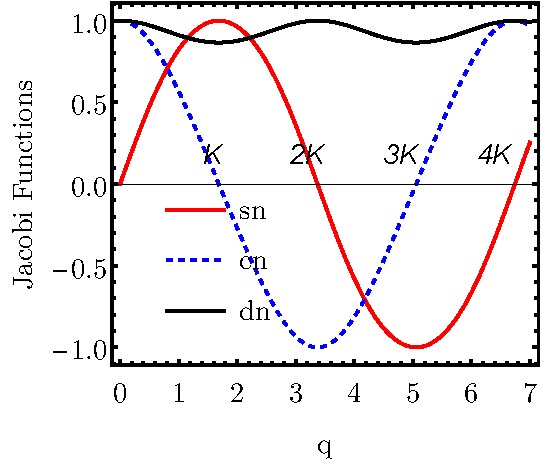
\includegraphics[scale=0.9]{Chapters/Figures/Jacobi-Elliptic-Functions.pdf}
    \caption{The elliptic functions sn, cd, and dn from Eq. \ref{elliptic-functions-equation} are represented as functions of $q$. The value of the \emph{elliptic modulus} $k$ is set to $1/2$.}
    \label{elliptic-functions-plot}
\end{figure}

Referring back to the angular momentum components, these can be written in terms of the elliptic functions and the variables $q$, $d/dq$ as such \cite{raduta2020new}:
\begin{align}
    \hat{I}_\pm&=i\frac{c\mp d}{k's}\left(I\pm\hat{I}_0\right)\ ,\nonumber\\
    \hat{I}_0&=Icd-s\frac{d}{dq}\ ,
    \label{angular-momentum-elliptic-representation}
\end{align}
which would make the Hamiltonian $\hat{H}'$ from Eq. \ref{hamiltonian-new-boson-ladder-operators} achieve the following shape:
\begin{align}
    \hat{H}'=-\frac{d^2}{dq^2}-2v_0s\frac{d}{dq}+I(I+1)s^2k^2+2v_0cdI\ .
\end{align}

By changing the wave-function $\ket{\Psi}$ to:
\begin{align}
    \ket{\Psi}=\left(d-kc\right)^{-\frac{v_0}{k}}\ket{\Phi}\ ,
\end{align}
the Schrödinger equation will have two fully separated \emph{kinetic} and \emph{potential} terms:
\begin{align}
    \left[-\frac{d^2}{dq^2}+V(q)\right]\ket{\Phi}=E\ket{\Phi}\ .
    \label{schrodinger-equation-elliptic}
\end{align}

The potential term $V(q)$ is defined as \cite{raduta2020new}:
\begin{align}
    V(q)=\left[I(I+1)k^2+v_0^2\right]s^2+\left(2I+1\right)v_0cd\ .
    \label{elliptic-potential-formula}
\end{align}
and it is graphically represented in Fig. \ref{elliptic-potential-plot}. It can be seen that $V(q)$ has a symmetry to the change of sign for the coordinate $q$. If the potential is calculated for the interval $q\in\left[-4K,4K\right]$, it has three deep symmetric wells, with degenerate minima, and two local minima surrounding $q=\pm 2K$. The states near the local minima are meta-stable, due to the tunneling effect making them transition to adjacent minima. These characteristics are illustrated in the set of Figs.
\begin{figure}
    \centering
    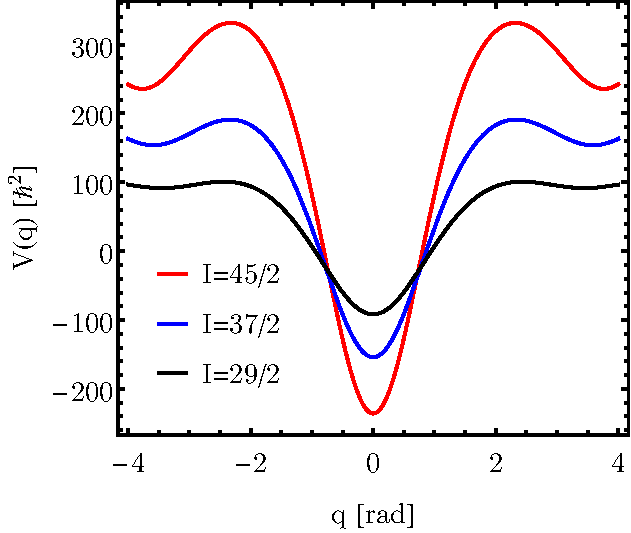
\includegraphics[scale=0.85]{Chapters/Figures/Elliptic-Potential-V.pdf}
    \caption{The potential energy as function of $q$ for several values of the angular momentum $I$. For the calculation of $V(q)$, the MOI were set to $\mathcal{I}_1:\mathcal{I}_2:\mathcal{I}_3=95:100:85\ \hbar\text{MeV}^{-2}$, $j=13/2$, and $\theta=-80^\circ$.}
    \label{elliptic-potential-plot}
\end{figure}
\begin{figure}
    \centering
    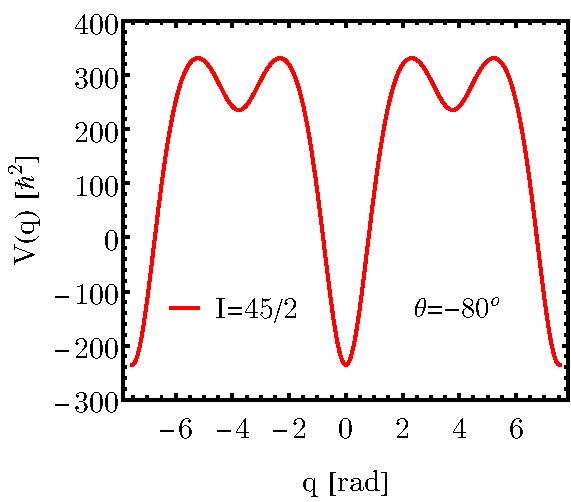
\includegraphics[width=0.49\textwidth]{Chapters/Figures/Elliptic-Potential-deep-1.pdf}
    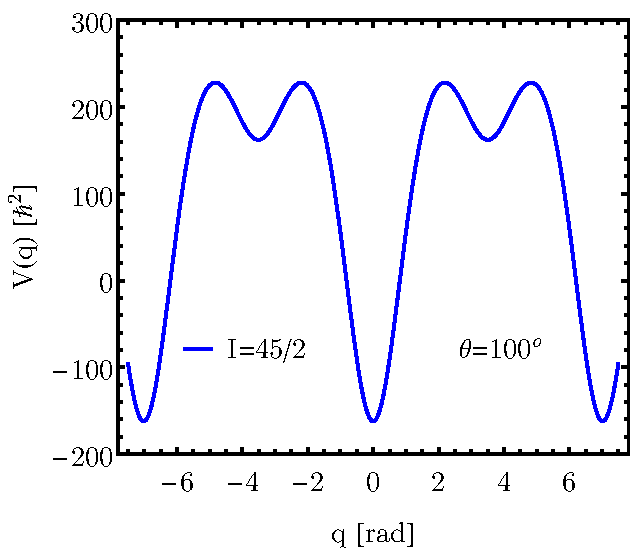
\includegraphics[width=0.49\textwidth]{Chapters/Figures/Elliptic-Potential-deep-1-180.pdf}
    \caption{The potential energy $V(q)$ for $\theta=-80^\circ$ and $\theta+\pi$, but for an extended range of the variable $q$, such that the deep and local minima can be seen. The same moments of inertia are used as in Fig. \ref{elliptic-functions-plot}.}
\end{figure}

Adopting the Bargmann representation, which was introduced in the previous section, for the angular momentum representation depicted in Eq. \ref{angular-momentum-elliptic-representation}, the three components $\hat{I}\mp$ and $\hat{I}_0$ become:
\begin{align}
    \hat{I}_+&=\iu\frac{cb^\dagger-db^\dagger}{k'sb^\dagger}\left(I+Icb^\dagger db^\dagger-sb^\dagger b\right)\ ,\nonumber\\
    \hat{I}_-&=\iu\frac{cb^\dagger+db^\dagger}{k'sb^\dagger}\left(I-Icb^\dagger d b^\dagger+sb^\dagger b\right)\ ,\nonumber\\
    \hat{I}_0&=Icb^\dagger db^\dagger-sb^\dagger b\ .
    \label{angular-momentum-elliptic-bargmann}
\end{align}

This is the first time in literature when such a transformation emerges. The boson expansion of the angular momentum components obtained from the elliptic functions $s$, $c$, $d$, and the Bargmann mapping applied on the same components is the remarking feature of the work from Ref. \cite{raduta2020new}. This expansion is different that the Dyson one, which was illustrated in Section \ref{section-intro-boson-representation}.

\subsection{Another boson expansion for the angular momentum}

When $k=0$, the following values are obtained for the elliptic functions:
\begin{align}
    q=\varphi\ ,\ d=1\ , K=\frac{\pi}{2}\ ,\ k'=1\ .
\end{align}

Using these values, the components from Eq. \ref{angular-momentum-elliptic-bargmann} can be re-written, such that in the rotating frame they become:
\begin{align}
    \hat{I}_+&=\iu\left[-I\sin b^\dagger+\left(1-\cos b^\dagger\right)b^\dagger\right]\ ,\nonumber\\
    \hat{I}_-&=\iu\left[I\sin b^\dagger+\left(1+\cos b^\dagger\right)b\right]\ ,\nonumber\\
    \hat{I}_0&=I\cos b^\dagger-b\sin b^\dagger\ ,
    \label{angular-momentum-new-expansion}
\end{align}
which can be simplified even more if the trigonometric functions are expanded and the leading terms are kept:
\begin{align}
    \hat{I}_+&=\iu\left[-Ib^\dagger+\frac{1}{2}b\left(b^\dagger\right)^2\right]\ ,\nonumber\\
    \hat{I}_-&=2\iu b\ ,\nonumber\\
    \hat{I}_0&=I-b^\dagger b\ .
    \label{angular-momentum-dyson-expansion}
\end{align}

The components from Eq. \ref{angular-momentum-dyson-expansion} are similar to the ones from the Dyson boson expansion (recall Eq. \ref{dyson-transformation}), making it clear now that the representations shown in Eq. \ref{angular-momentum-elliptic-bargmann} and Eq. \ref{angular-momentum-new-expansion} are in fact generalizations of the Dyson representation.

\subsection{Harmonic Approximation of the Energy}

One can aim at solving numerically Eq. \ref{schrodinger-equation-elliptic}, but there could be a rather simpler and more \emph{elegant} approach to this. Adopting the harmonic approximation (as described in the previous chapters) can provide valid results. First step is to analyze the stationary points of the elliptic potential $V(q)$. Its first order derivative is given by \cite{raduta2020new}:
\begin{align}
    \frac{d}{dq}V(q)=s\left[\left(I(I+1)k^2+v_0^2\right)2cd-(2I+1)v_0k'^2-(2I+1)v_02k^2c^2\right]\ .
\end{align}

There are five minima, located at $q=0,\pm2K,\pm4K$. Remarkable that for $q=\pm2K$ the two minima emerge for angular momentum values that are lager than $19/2$. This is emphasized in Fig. \ref{elliptic-potential-plot-2k-minima}, where it can be seen that the minima are flat at the beginning, but their depth increases with increasing values of $I$.
\begin{figure}
    \centering
    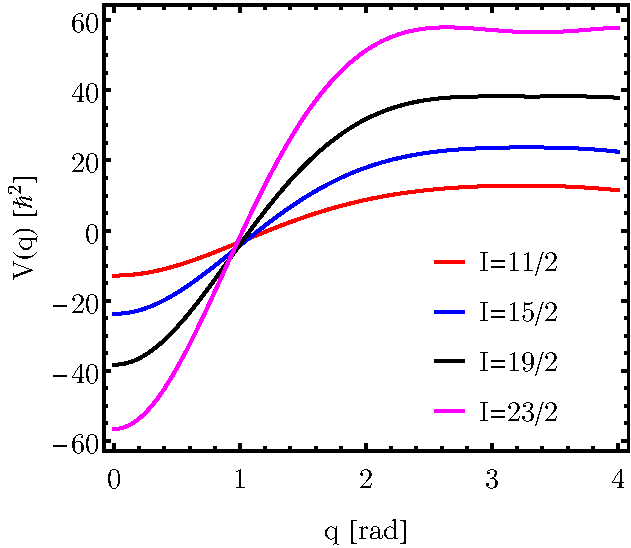
\includegraphics[scale=0.85]{Chapters/Figures/Elliptic-Potential-2K-Minima.pdf}
    \caption{The potential $V(q)$ from Eq. \ref{elliptic-potential-formula}, near the $q=2K$ minimum point. It can be observed that the minimum character appears only for $I>19/2$.}
    \label{elliptic-potential-plot-2k-minima}
\end{figure}

The angular momentum can be studied in terms of its orientation near the minimum points. This is achieved if the boson expansion is written as \cite{raduta2020new}:
\begin{align}
    \hat{I}_+&=\frac{\iu}{k'}\left[I\left(-d+ck^2\right)s-(c-d)\frac{d}{dq}\right]\ ,\nonumber\\
    \hat{I}_-&=\frac{\iu}{k'}\left[I\left(d+ck^2\right)s+(c+d)\frac{d}{dq}\right]\ ,\nonumber\\
    \hat{I}_0&=Icd-s\frac{d}{dq}\ ,
\end{align}
and for $q=\pm2K$ (that is $\varphi=\pm\pi$) one has $\hat{I}_0=-I$, while $q=0$ (i.e., $\varphi=2$) will lead to $\hat{I}_0=I$. Consequently, in the local minima the total angular momentum will align anti-parallel with the $1$-axis, and for the deep minimum $q=0$ the angular momentum is aligned along the (1)-axis. Expanding the elliptic potential $V(q)$ up to second order in the coordinate, an equation that looks similar to the harmonic oscillator is obtained for the Hamiltonian $\hat{H}_\text{rot}$ (firstly introduced in Eq. \ref{rotor-hamiltonian-new-boson}):
\begin{align}
    E_n=A_1I^2+\hbar\omega\left(n+\frac{1}{2}\right)+e_\text{sp}\ ,
    \label{energy-2nd-order-expansion-deepest-minima}
\end{align}
where the single-particle term is defined as:
\begin{align}
    e_\text{sp}=\sum_{i=1,2}A_ij_i^2-(2I+1)A_1j_1-IA_2j_2\ .
\end{align}

The frequency $\omega$ from Eq. \ref{energy-2nd-order-expansion-deepest-minima} has the expression:
\begin{align}
    \omega^2=&\left[(2I+1)\left(A_2-A_1-\frac{A_2j_2}{I}\right)+2A_1j_1\right]\cdot\nonumber\\
                &\cdot\left[(2I+1)(A_3-A_1)+2A_1j_1\right]-(A_3-A_1)\left(A_2-A_1-\frac{A_2j_2}{I}\right)\ .
    \label{omega-frequency-deepest-minima}
\end{align}

On the other hand, if the potential is expanded around the local minimum $q=2K$, and only the quadratic terms are kept, then the following set of energies :
\begin{align}
    E_n^{(2K)}&=-(2I+1)v_0+\hbar\omega^{(2K)}\left(n+\frac{1}{2}\right)\ ,\nonumber\\
    \left(\omega^{(2K)}\right)^2&=\left(1+\frac{2v_0}{2I+1}\right)\left(u+\frac{2v_0}{2I+1}\right)(2I+1)^2-u\ ,
\end{align}

The Hamiltonian $\hat{H}_\text{rot}$ is connected to $\hat{H}'$ via Eq. \ref{rewritten-rotor-hamiltonian-new-boson}, meaning that the final energy spectrum of $\hat{H}'$ will be given by:
\begin{align}
    E_n'&=A_1I^2+\hbar\omega'\left(n+\frac{1}{2}\right)+e_\text{sp}\ ,\nonumber\\
    e_\text{sp}&=\sum_{i=1,2}A_ij_i^2-(2I+1)A_1j_1-IA_2j_2\ ,
\end{align}
with the wobbling frequency $\omega'$ having the following definition:
\begin{align}
    \omega'^2=&\left[(2I+1)\left(A_2-A_1-\frac{A_2j_2}{I}\right)-2A_1j_1\right]\left((2I+1)(A_3-A_1)-2A_1j_1\right)-\nonumber\\
    &-(A_3-A_1)\left(A_2-A_1-\frac{A_2j_2}{I}\right)
    \label{wobbling-frequency-new-boson-prime}
\end{align}

The two wobbling frequencies, i.e., $\omega$ and $\omega'$ are both graphically represented in Fig. \ref{wobbling-frequencies-harmonic-approx}. As the angular momentum components $j_1$ and $j_2$ depend on the angle $\theta$, the evolution of both frequencies is plotted as function of this coordinate. It can be seen from the two curves that both wobbling frequencies have a maximum value $\approx1$, but $\omega_\text{max}$ is located at $\theta\approx-0.7\ \text{rad}$, while $\omega'_\text{max}$ is at $\theta\approx-2.4\ \text{rad}$. Moreover, the two frequencies intersect each other at the points $\theta=-\pi/2$ and $\theta=\pi/2$.
\begin{figure}
    \centering
    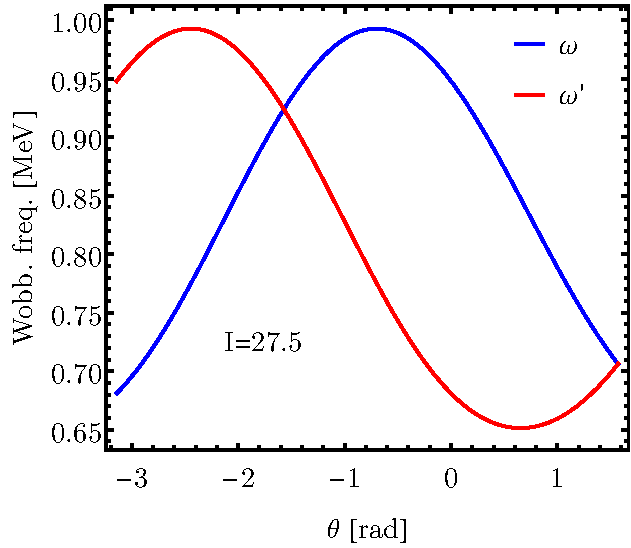
\includegraphics[scale=0.85]{Chapters/Figures/Wobbling-Frequencies-New-Boson.pdf}
    \caption{The two wobbling frequencies $\omega$ (Eq. \ref{omega-frequency-deepest-minima}) and $\omega'$ (Eq. \ref{wobbling-frequency-new-boson-prime}) as function of the coordinate $\theta$ for a fixed set of MOI $\mathcal{I}_1:\mathcal{I}_2:\mathcal{I}_3=91:9:51\ \hbar^2\text{MeV}^{-1}$ and single-particle angular momentum $j=13/2$.}
    \label{wobbling-frequencies-harmonic-approx}
\end{figure}

\section{A Classical Description of the Hamiltonian}
\label{classical-description-new-boson-section}

Going further with the analysis performed in Ref. \cite{raduta2020new}, the quantal operators associated to the angular momentum are dequantized, through the algebra:
\begin{align}
    [\ ,\ ] \longrightarrow -\iu\{\ ,\ \}\ ,
\end{align}
where the Poisson brackets replacing the commutator. The dequantization procedure consists of replacing the operators $\hat{I}_k$ with the classical components of the angular momentum (i.e., $I_k$. The conjugate coordinate of $I_k$ are further denoted by $\varphi_k$ and the three angular momentum components $I_k$ are hereafter denoted by $x_k$. With this algebra, the quantal Hamiltonian from Eq. \ref{new-boson-hamiltonian-notations} will be equivalent to:
\begin{align}
    H'=x_2^2+ux_3^2+2v_0I_x\ .
    \label{new-boson-h-prime-classical}
\end{align}

The equations of motion for $H'$ are (time derivatives are specified by the dot symbol):
\begin{align}
    \dot{x}_1&=2(1-v)x_2x_3\ ,\nonumber\\
    \dot{x}_2&=2(x_1u-v_0)x_3\ ,\nonumber\\
    \dot{x}_3&=-2(x_1-v_0)x_2\ .
\end{align}

The two constants of motion for this classical problem are:
\begin{align}
    E=x_2^2+ux_3^2+2v_0x_1\ ,
\end{align}
and 
\begin{align}
    I^2=x_1^2+x_2^2+x_3^2\ ,
\end{align}
which is in complete agreement with the fact the total energy and the total angular momentum are conserved.

Now that the classical counterpart of $\hat{H}'$ is analytically obtained, there can be several situations that can lead to the description of the harmonic-lie motion of the even-odd system. Namely, by considering the three angular momentum components $x_1$, $x_2$, and $x_3$ in the \emph{polar coordinate system} (defined by the coordinates $\theta$ and $\varphi$), one can have multiple considerations. These will be discussed below.

\subsubsection*{Case A1}

The maximal MOI corresponds to the $2$-axis. The Cartesian coordinates are changed to the polar ones via:
\begin{align}
    x_2=I\cos\theta_2\ ,\ x_3=I\sin\theta_2\cos\varphi_2\ ,\ x_1=I\sin\theta_2\sin\varphi_2\ .
    \label{polar-coordinates-case-a1}
\end{align}

The energy function $H'$ can be expressed in terms of the conjugate coordinates $(x_2,\varphi_2)$:
\begin{align}
    H'=x_2^2\left(1-u\cos^2\varphi_2-\frac{v_0}{I}\sin\varphi_2\right)+uI^2\cos^2\varphi_2+2v_0I\sin\varphi_2\ .
    \label{classical-energy-new-boson-2-axis}
\end{align}
This function has a minimum value of $H'\vert_\text{min}=-2v_0I$ at $(x_2,\varphi_2)=(0,-\pi/2)$, and the second derivatives for $H'$ in that point are:
\begin{align}
    \left.\frac{\partial^2H'}{\partial x_2^2}\right\vert_\text{min}&=2\left(2+\frac{v_0}{I}\right)\ ,\nonumber\\
    \left.\frac{\partial^2 H'}{\partial \varphi_2^2}\right\vert_\text{min}&=2\left(u+\frac{v_0}{I}\right)I^2\ .
\end{align}

If the classical energy function is expanded up to second order around the minimum point, then $H'$ will look like:
\begin{align}
    H'^{(2)}=-2v_0I\left(1+\frac{v_0}{I}\right)\bar{x}_2^2+\left(u+\frac{v_0}{I}\right)I^2\bar{\varphi}_2^2\ ,
\end{align}
where the deviation of the coordinates from the minimum point was denoted by $(\bar{x}_2,\bar{\varphi}_2)$ and the superscript $(2)$ suggests the second order expansion. This kind of function describes an oscillator with the frequency:
\begin{align}
    \omega^{(2)}=2\sqrt{(I+v_0)(Iu+v_0)}\ .
\end{align}

In the minimum point, the angular momentum components are $(x_1,x_2,x_3)=(-I,0,0)$ and $E=-2v_0I$. In Fig. \ref{energy-function-comparison-a1-case} the energy function $H'$ is graphically represented for $x_2=0$ and $\varphi_2=-\pi/2$, respectively, by keeping one coordinate fixed and varying the other. On both plots, the minimum value for $H'$ is achieved at the value $-2Iv_0$.
\begin{figure}
    \centering
    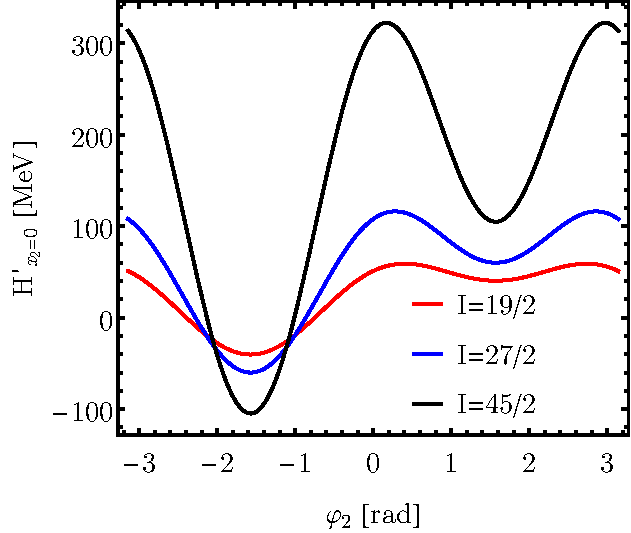
\includegraphics[width=0.49\textwidth]{Chapters/Figures/Energy-Function-New-Boson-A1-x2-const.pdf}
    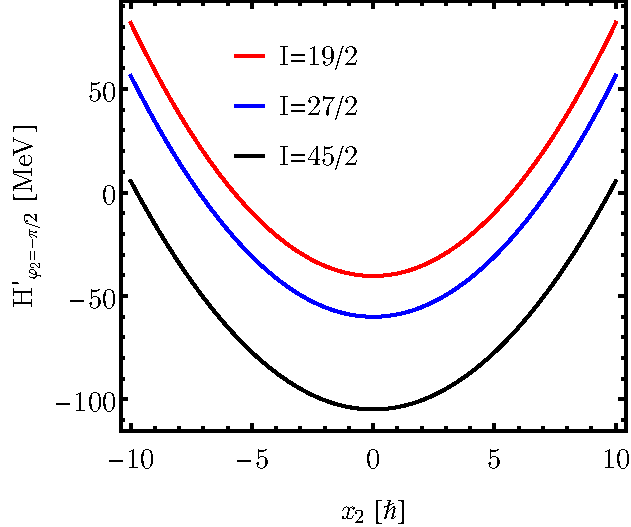
\includegraphics[width=0.49\textwidth]{Chapters/Figures/Energy-Function-New-Boson-A1-phi2-const.pdf}
    \caption{The classical energy $H'$ from Eq. \ref{classical-energy-new-boson-2-axis} evaluated for a fixed $x_2=0$ (left) and fixed $\varphi_2=-\pi/2$ (right). The calculations were done for $\mathcal{I}_1:\mathcal{I}_2:\mathcal{I}_3=10:40:20\ \hbar\text{MeV}^{-1}$. The single-particle angular momentum $j=11/2$.}
    \label{energy-function-comparison-a1-case}
\end{figure}

\subsubsection*{Case A2}

Another minimum point for $H'$ is $(0,\pi/2)$, in which the angular momentum is $(x_1,x_2,x_3)=(I,0,0)$ and the energy is $E=2v_0I$. Repeating the second order expansion for $H'$, the following formula is attained:
\begin{align}
    H'^{(2)}=2v_0I+\left(1-\frac{v_0}{I}\right)\bar{x}_2^2+I^2\left(u-\frac{v_0}{I}\right)\bar{\varphi}_2^2\ ,
\end{align}
which describes a harmonic oscillator with a frequency:
\begin{align}
    % \omega^{(2)}=2\sqrt{\left(1-\frac{v_0}{I}\right)\left(u-\frac{v_0}{I}\right)I^2}\ .
    \omega^{(2)}=2\sqrt{(I-v_0)(uI-v_0)}\ .
\end{align}

\subsubsection*{Case A3}

A third set of conjugate variables for which $H'$ is minimal is: $$(x_2,\varphi_2)=(0,\arcsin\left(\frac{v_0}{Iu}\right))\ .$$ With this set of coordinates the energy function will become after expansion:
\begin{align}
    H'^{(2)}=uI^2+\frac{v_0^2}{u}+(1-u)\bar{x}_2^2-u\left(I^2-\frac{v_0^2}{u^2}\right)\bar{\varphi}_2^2\ .
\end{align}

For a positive value of $u$, but confined inside $u\in(0,1)$ the coordinates consist of a \emph{saddle point} with angular momentum components: $$(x_1,x_2,x_3)=\left(\frac{v_0}{u},0,\sqrt{I^2-\frac{v_0^2}{u^2}}\right)\ ,$$ and energy: $$E=I^2u+\frac{v_0^2}{u}\ .$$

Summarizing the situations $A1$, $A2$, and $A3$, there are three stationary points for $H'$ when the maximal MOI is along the $2$-axis, (i.e., the quantization axis). The points are provided in Table \ref{stationary-points-2-axis}, where values for $x_2$ and $\varphi_2$ are accompanied by the angular momentum components and the value of the energy. Moreover, the character of each stationary point is also mentioned.
\begin{table}
    \centering
    \resizebox{\textwidth}{!}{%
    \begin{tabular}{|c|c|c|c|c|c|}
    \hline
    \multicolumn{1}{|c|}{Point $p$} &
    \multicolumn{1}{c|}{$x_2$} &
    \multicolumn{1}{c|}{$\varphi_2$} &
    \multicolumn{1}{c|}{\begin{tabular}[c]{@{}c@{}}A.m. components\\ $(x_1,x_2,x_3)$\end{tabular}} &
    \multicolumn{1}{c|}{$E$} &
    \multicolumn{1}{c|}{\begin{tabular}[c]{@{}c@{}}Character \\ of the stationary point\end{tabular}} \\ \hline
    $p_0(m)$ & $0$ &  $-\frac{\pi}{2}$    & $(-I,0,0)$ & $E=-2v_0I$ & minimum (m) \\
    $p_1(m)$ & $0$ &  $\frac{\pi}{2}$    & $(I,0,0)$ & $E=2v_0I$ & minimum (m) \\
    $p_2(s)$ & $0$ &  $\arcsin\left(\frac{v_0}{Iu}\right)$  & $\left(\frac{v_0}{u},0,\sqrt{I^2-\frac{v_0^2}{u^2}}\right)$ & $E=\left(I^2u+\frac{v_0^2}{u}\right)$ & saddle (s)\\
    \hline
    \end{tabular}%
    }
    \caption{The stationary points for the classical energy function depicted in Eq. \ref{new-boson-h-prime-classical}, when the quantization axis is the $2$-axis. Each point corresponds to the cases $A1$, $A2$, and $A3$, respectively.}
    \label{stationary-points-2-axis}
\end{table}

Considering that the polar coordinates used to define the three angular momentum components can be replaced in the expression of $H'$ from Eq. \ref{new-boson-h-prime-classical}, then an energy function that will depend explicitly $\theta_2$ and $\varphi_2$. This \emph{polar representation of the classical energy function} can be represented for a given interval of $\theta_2$ and $\varphi_2$, respectively. Fixing the total angular momentum $I$, the single-particle a.m. $j$, the three MOI, and the value of $\theta$ (not to be confused with the polar $\theta_2$), a contour plot such as the one shown in Fig. \ref{new-boson-hprime-2axis-contour-plot} can be obtained. Within the contour plot, there are several stationary points: one deep minimum, one local minimum, and two saddle points. Every point lies along the $\theta_2=\pi/2$ coordinate. In order to better perceive how the minima and saddle points are located, Fig. \ref{new-boson-hprime-2axis-varphi-plot} shows the evolution of $H'$ for $\theta_2=\pi/2$. Keep in mind that both figures are evaluated for the same set of constants.
\begin{figure}
    \begin{center}
        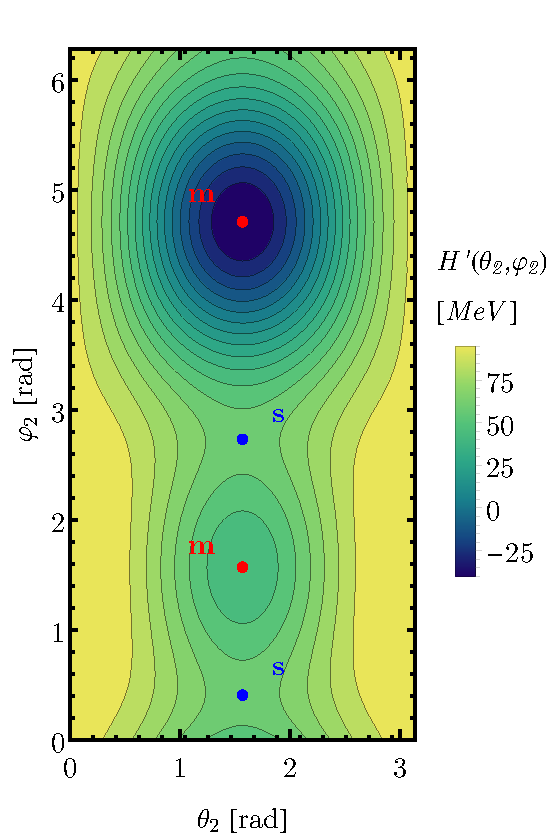
\includegraphics[scale=0.7]{Chapters/Figures/New-Boson-Classical-H-2axis-quantization.pdf}
        \caption{Contour plot for the energy $H'$ from Eq. \ref{new-boson-h-prime-classical}, defined in terms of the polar coordinates. The calculations are done for the A1-A2-A3 cases (i.e., maximal MOI is $\mathcal{I}_2)$. The single-particle angular momentum is $j=11/2$, the total angular momentum $I=19/2$, the MOIs are $\mathcal{I}_1:\mathcal{I}_2:\mathcal{I}_3=10:40:20\ \hbar^2\text{MeV}^{-1}$, and $\theta=70^\circ$. The four stationary points are illustrated, namely two minima - one local and one global - (denoted by "m") and two saddle points (denoted by "s").}
        \label{new-boson-hprime-2axis-contour-plot}
    \end{center}
\end{figure}
\begin{figure}
    \begin{center}
        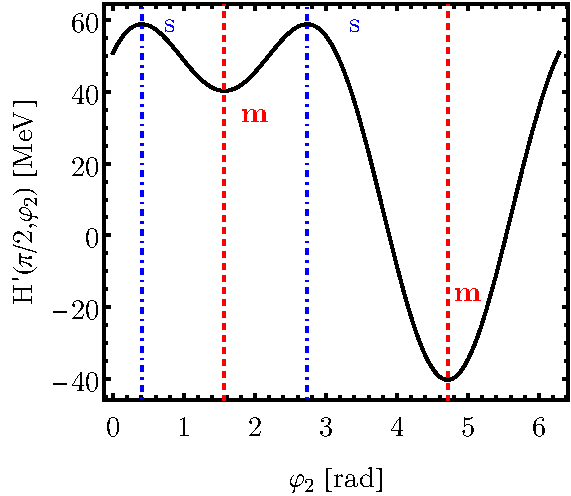
\includegraphics[scale=0.8]{Chapters/Figures/New-Boson-Classical-H-2-axis-varphi-plot.pdf}
        \caption{The classical energy $H'$ from Eq. \ref{new-boson-h-prime-classical}, for a fixed $\theta_2=\pi/2$ and $\varphi\in[0,2\pi]$. The single-particle angular momentum is $j=11/2$, the total angular momentum $I=19/2$, the MOIs are $\mathcal{I}_1:\mathcal{I}_2:\mathcal{I}_3=10:40:20\ \hbar^2\text{MeV}^{-1}$, and $\theta=70^\circ$. The critical points present in Fig. \ref{new-boson-hprime-2axis-contour-plot} are also illustrated here by the dashed vertical lines (two minima with red color and two saddle points with blue color).}
        \label{new-boson-hprime-2axis-varphi-plot}
    \end{center}
\end{figure}

\subsubsection*{Case B1}

Going further with the analysis, a second approach would be to consider the $3$-axis as the quantization axes, meaning that now the largest MOI is around this axis. The angular momentum components written in terms of the polar coordinates $(\theta_3,\varphi_3)$ will be defined in the following way:
\begin{align}
    x_1=I\sin\theta_3\cos\varphi_3\ ,\ x_2=I\sin\theta_3\sin\varphi_3\ ,\ x_3=I\cos\theta_3\ ,
    \label{polar-coordinates-case-b1}
\end{align}

In the same way as the $A$-cases. the total energy $H'$ can be expressed in terms of the $x_3$ coordinate and the polar $\varphi_3$ one:
\begin{align}
    H'^{(2)}=x_3^2\left(u-\sin^2\varphi_3-\frac{v_0}{I}\cos\varphi_3\right)+I^2\sin^2\varphi_3+2v_0I\cos\varphi_3\ .
    \label{classical-energy-new-boson-3-axis}
\end{align}

The first stationary point of Eq. \ref{classical-energy-new-boson-3-axis} with a minimum character is $(x_3,\varphi_3)=(0,\pi)$. For this point, the angular momentum components are $(x_1,x_2,x_3)=(-I,0,0)$, hinting to the fact that the total a.m. is oriented along the one-axis. The value of the energy in this point is $E=-2v_0I$. The harmonic Hamiltonian given in the second order expansion around this point is:
\begin{align}
    H'^{(2)}=-2v_0I+\left(u+\frac{v_0}{I}\right)\bar{x}_3^2+I^2\left(1+\frac{v_0}{I}\right)\bar{\varphi}_3^2\ ,
\end{align}

having a similar shape for the wobbling frequency as per $A1$ case. Similarly as for $A1$ case, the Hamiltonian $H'$ is also represented  in terms of only one coordinate at a time, where each of the coordinates are fixed to $x_3=0$ and $\varphi_3=\pi$, respectively. These plots are shown in Figs. \ref{energy-function-comparison-b1-case}.
\begin{figure}
    \centering
    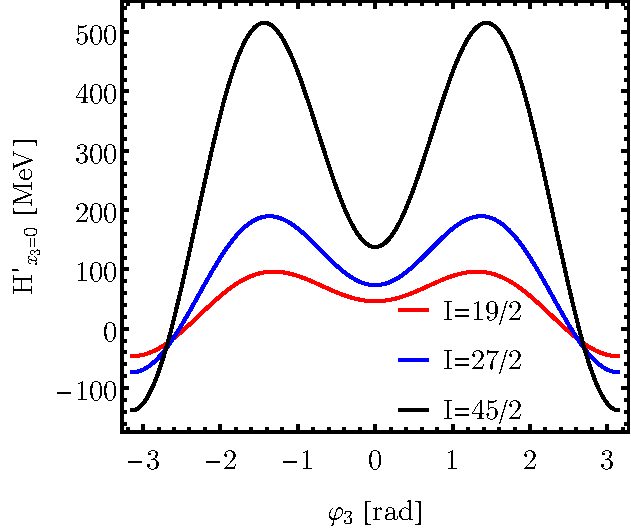
\includegraphics[width=0.49\textwidth]{Chapters/Figures/Energy-Function-New-Boson-B1-x3-const.pdf}
    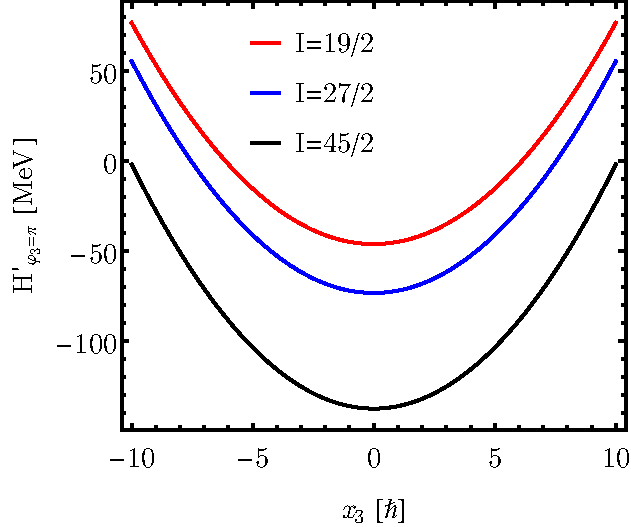
\includegraphics[width=0.49\textwidth]{Chapters/Figures/Energy-Function-New-Boson-B1-phi3-const.pdf}
    \caption{The classical energy $H'$ from Eq. \ref{classical-energy-new-boson-3-axis} evaluated for a fixed $x_3=0$ (left) and fixed $\varphi_3=\pi$ (right). The calculations were done for $\mathcal{I}_1:\mathcal{I}_2:\mathcal{I}_3=10:20:40\ \hbar\text{MeV}^{-1}$. The single-particle angular momentum $j=11/2$.}
    \label{energy-function-comparison-b1-case}
\end{figure}

\subsubsection*{B2 case}

Another stationary point for Eq. \ref{classical-energy-new-boson-3-axis} is $(x_3,\varphi)=(0,0)$, which is also a minimum. The second order expansion of $H'$ gives:
\begin{align}
    H'=2v_0I+\left(u-\frac{v_0}{I}\right)\bar{x}_3^2+I^2\left(1-\frac{v_0}{I}\right)\bar{\varphi}_3^2\ ,
\end{align}
and moreover $(x_1,x_2,x_3)=(I,0,0)$, and $E=2v_0I$. The wobbling frequency is:
\begin{align}
    \omega^{(2)}=2\sqrt{\left(1-\frac{v_0}{I}\right)\left(u-\frac{v_0}{I}\right)I^2}\ .
\end{align}

\subsubsection*{B3 case}

Lastly, the stationary point $(x_3,\varphi_3)=\left(0,\arccos\frac{v_0}{I}\right)$ is a maximum, giving a.m. components:
\begin{align}
    (x_1,x_2,x_3)=\left(v_0,\sqrt{I^2-v_0^2},0\right)\ ,
\end{align}
and energy $E=I^2+v_0^2\ .$ For this maximum point, the energy function $H'$ becomes:
\begin{align}
    H'^{(2)}=I^2+v_0^2+\left(u-1\right)\bar{x}_3^2+\left(v_0^2-I^2\right)\bar{\varphi}_3^2\ .
\end{align}

The contour plot of the energy function $H'$ can be obtained in the same manner as for $A$ situations, i.e., taking the polar coordinates $(\theta_3,\varphi_3)$ that are used in the expression of the angular momentum components from Eq. \ref{polar-coordinates-case-b1}, and evaluate $H'(\theta_3,\varphi_3)$ for fixed values of $j,\ I,\ \mathcal{I}_1,\ \mathcal{I}_2,\ \mathcal{I}_3$, and $\theta$. The contour plot together with the evolution of $H'(\pi,\varphi_3)$ are drawn in Figs. \ref{new-boson-hprime-3axis-contour-plot} - \ref{new-boson-hprime-3axis-varphi-plot}. Therein, five stationary points can be observed: two maxima denoted by "M" (magenta color) and three minima denoted by "m" (red color).
\begin{figure}
    \begin{center}
        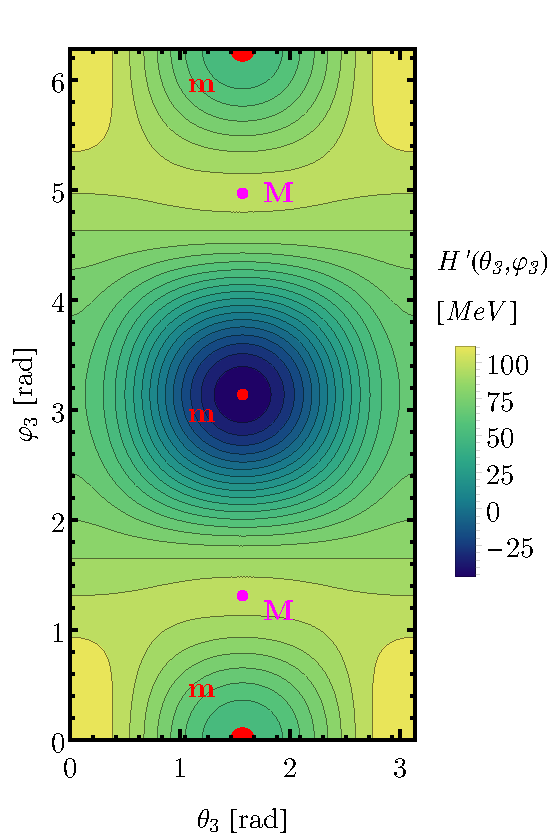
\includegraphics[scale=0.7]{Chapters/Figures/New-Boson-Classical-H-3axis-quantization.pdf}
        \caption{Contour plot for the energy $H'$ from Eq. \ref{new-boson-h-prime-classical}, defined in terms of the polar coordinates. The calculations are done for the B1-B2-B3 cases (i.e., maximal MOI is $\mathcal{I}_3)$. The single-particle angular momentum is $j=11/2$, the total angular momentum $I=19/2$, the MOIs are $\mathcal{I}_1:\mathcal{I}_2:\mathcal{I}_3=10:20:40\ \hbar^2\text{MeV}^{-1}$, and $\theta=70^\circ$. The five stationary points are illustrated, namely two maxima (denoted by "M") and three minimum points (denoted by "m"; one global and two local).}
        \label{new-boson-hprime-3axis-contour-plot}
    \end{center}
\end{figure}
\begin{figure}
    \begin{center}
        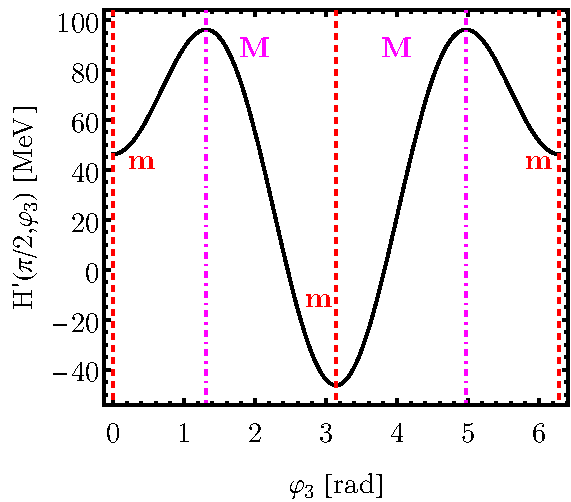
\includegraphics[scale=0.8]{Chapters/Figures/New-Boson-Classical-H-3-axis-varphi-plot.pdf}
        \caption{The classical energy $H'$ from Eq. \ref{new-boson-h-prime-classical}, for a fixed $\theta_2=\pi/2$ and $\varphi\in[0,2\pi]$. The single-particle angular momentum is $j=11/2$, the total angular momentum $I=19/2$, the MOIs are $\mathcal{I}_1:\mathcal{I}_2:\mathcal{I}_3=10:20:40\ \hbar^2\text{MeV}^{-1}$, and $\theta=70^\circ$. The critical points present in Fig. \ref{new-boson-hprime-3axis-contour-plot} are illustrated by the dashed vertical lines (magenta for the maxima and red for the minima).}
        \label{new-boson-hprime-3axis-varphi-plot}
    \end{center}
\end{figure}

\subsubsection*{Case C1}

Lastly, the situation when the largest MOI corresponds to the $1$-axis should be analyzed. Choosing thus $1$-axis as the quantization axis, the a.m. components are (in polar coordinates):
\begin{align}
    x_1=I\cos\theta_1\ ,\ x_2=I\sin\theta_1\cos\varphi_1\ ,\ x_3=I\sin\theta_1\sin\varphi_1,
    \label{polar-coordinates-case-c1}
\end{align}
with the associated Hamiltonian:
\begin{align}
    H'=\left(I^2-x_1^2\right)\left(\cos^2\varphi_1+u\sin^2\varphi_1\right)+2v_0x_1\ .
    \label{classical-energy-new-boson-1-axis}
\end{align}

The Hamiltonian from Eq. \ref{classical-energy-new-boson-1-axis} has a stationary point at $(x_1,\varphi_1)=\left(\frac{v_0}{u},\frac{\pi}{2}\right)$. This is a \emph{saddle} point when $u\in(0,1)$. The second order expansion of $H'$ is therefore:
\begin{align}
    H'^{(2)}=uI+\frac{v_0}{u}-u\bar{x}_1^2+(1-u)\left(I^2-\frac{v_0^2}{u^2}\right)\bar{\varphi}_1^2\ .
\end{align}

\subsubsection*{Case C2}

The last stationary point is a maximum, given by the coordinates $(v_0,0)$, for which the a.m. components are: $$(x_1,x_2,x_3)=(v_0,\sqrt{I^2-v_0^2},0)\ ,$$ and the energy $E=I^2+v_0^2$. The Hamiltonian up to second order becomes:
\begin{align}
    H'^{(2)}=I^2+v_0^2-\bar{x}_1^2+(u-1)\left(I^2-v_0^2\right)\bar{\varphi}_1^2\ .
\end{align}

In Fig. \ref{new-boson-hprime-1axis-contour-plot}, a contour plot with the energy function from Eq. \ref{classical-energy-new-boson-1-axis} is shown, where three maxima and two saddle points are present. The calculation of $H'(\theta_1,\varphi_1)$ used a different set of MOI than the A-B cases. Namely, $\mathcal{I}_1:\mathcal{I}_2:\mathcal{I}_3=80:10:50\ \hbar^2\text{MeV}^{-1}$, but $\theta$ was kept identical. The maxima from Fig \ref{new-boson-hprime-1axis-contour-plot} would illustrate that a rotation around the $1$-axis (the cranking axis for the initial system) is not possible.
\begin{figure}
    \begin{center}
        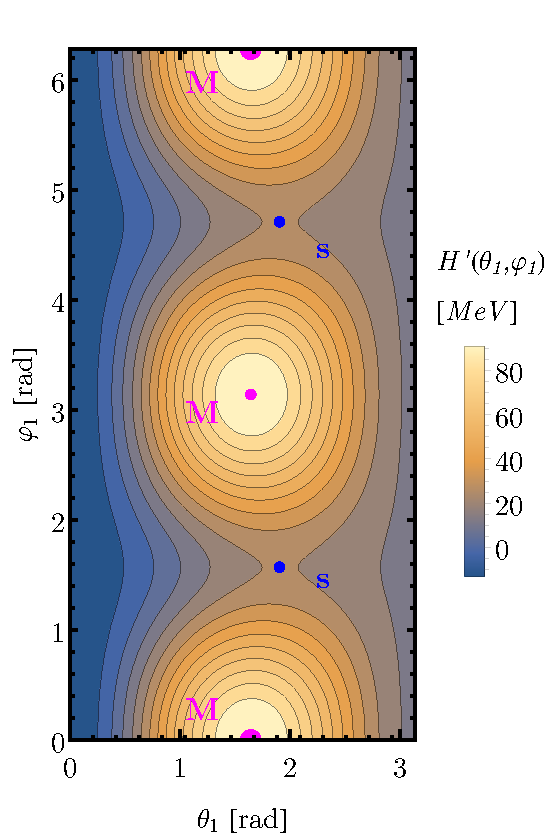
\includegraphics[scale=0.7]{Chapters/Figures/New-Boson-Classical-H-1axis-quantization.pdf}
        \caption{Contour plot for the energy $H'$ from Eq. \ref{new-boson-h-prime-classical}, defined in terms of the polar coordinates. The calculations are done for $\mathcal{I}_1:\mathcal{I}_2:\mathcal{I}_3=80:10:50\ \hbar^2\text{MeV}^{-1}$ (i.e., the $1$-axis is the quantization axis). The single-particle angular momentum is $j=11/2$, the total angular momentum $I=19/2$, and $\theta=70^\circ$. The five stationary points are illustrated, namely three maxima (denoted by "M") and two saddle points (denoted by "s").}
        \label{new-boson-hprime-1axis-contour-plot}
    \end{center}
\end{figure}
